\documentclass[11pt]{article}
\usepackage{fullpage,amsmath,amsfonts,mathpazo,microtype,nicefrac,graphicx,verbatimbox,listings,hyperref,enumitem,amssymb,float,fancyhdr}

% Margins
% \topmargin=-0.45in
% \evensidemargin=0in
% \oddsidemargin=0in
% \textwidth=6.5in
% \textheight=9.0in
% \headsep=0.25in

% \linespread{1.1} % Line spacing

% % Set up the header and footer
% \pagestyle{fancy}
% \lhead{\hmwkAuthorName} % Top left header
% \chead{\hmwkClass\ (\hmwkClassInstructor\ \hmwkClassTime): \hmwkTitle} % Top center header
% \rhead{\firstxmark} % Top right header
% \lfoot{\lastxmark} % Bottom left footer
% \cfoot{} % Bottom center footer
% \rfoot{Page\ \thepage\ of\ \pageref{LastPage}} % Bottom right footer
% \renewcommand\headrulewidth{0.4pt} % Size of the header rule
% \renewcommand\footrulewidth{0.4pt} % Size of the footer rule

% \setlength\parindent{0pt} % Removes all indentation from paragraphs

%----------------------------------------------------------------------------------------
%   TITLE PAGE
%----------------------------------------------------------------------------------------

\title{
\vspace{1cm}
\textmd{\textbf{AC209a Milestone 5: Data Science with User Ratings and Reviews}}\\
% \normalsize\vspace{0.1in}\small{Due\ on\ \hmwkDueDate}\\
% \vspace{0.1in}\large{\textit{\hmwkClassInstructor\ \hmwkClassTime}}
}

\author{\textbf{Andrew Ross, Sophie Hilgard, Reiko Nishihara, Nick Hoernle}}
\date{\today} % Insert date here if you want it to appear below your name

%----------------------------------------------------------------------------------------

\begin{document}

\maketitle

\section*{Proposal of Future Work}
\paragraph{} 	For Baseline Models in Milestone 4, we have implemented simple averaging as well as basic content-based recommendations and collaborative filtering models. Going forward, we hope to build more sophisticated models within these classes. In particular, we will explore creating a hybrid collaborative filtering/matrix factorization model or a model which more heavily weights recent ratings.
\paragraph{}	We also built a network-based recommendation system based roughly on the PageRank algorithm. This model finds the most `connected` business, where path lengths between businesses are weighted inversely to how much a user liked both of the restaurants. To find the next recommendation for any given user, we search the graph built off of similar users and return the `closest` business the user has not yet been to.
\paragraph{}	We have also explored a number of other models for predicting business success rather than focusing only on recommendation systems. In particular, we have spent time focusing on other aspects within the yelp challenge that ask you to predict business success based on location or investigate seasonal and otherwise temporal trends in business popularity. Location based models have focused largely on clustering methods, as neighborhood is a better predictor than absolute latitude and longitude values. Trend analysis will use regression models over time to analyze if businesses are cyclically  popular at any given lag or to find points in time when a given business was comparatively `hot` within its lifetime.
\paragraph{}
Lastly, we have been aiming to determine how location and seasonal trends alone impact the reviewers mindset (and consequently the reviews that they give to a business). To do this, we have used a time series analysis visualization (shown in figure \ref{fg:bars_nightlife}) to highlight any repetitive trends that may be present in the data. For example the plot below shows the ratings that are above the mean in red and the ratings that are below the mean in blue. The average number of ratings per day of the week is shown in the right side vertical axis and the number of ratings on any one day of the year is shown in the axis above the plot. We clearly see that the reviews that are given on Sundays and Mondays tends to be more positive than the reviews given on the other days of the week.
\begin{figure}[H]
\centering
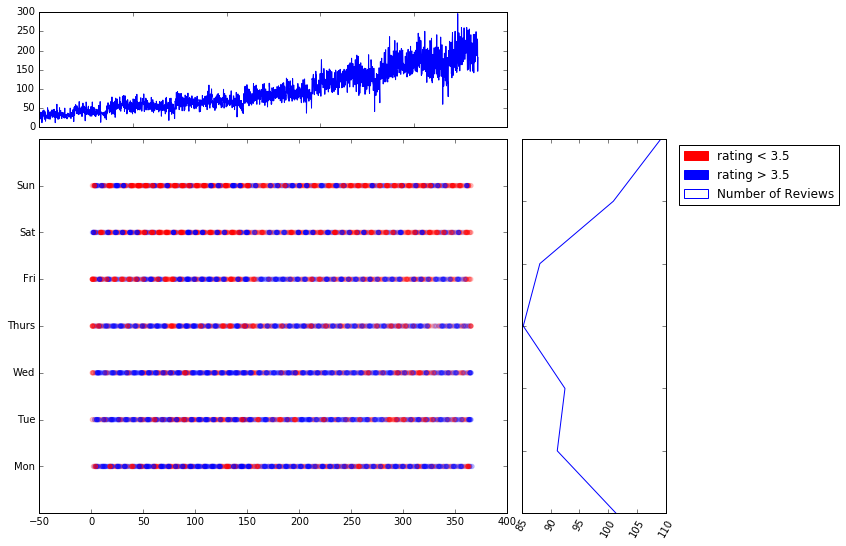
\includegraphics[keepaspectratio=true,scale=0.4]{./images/bars_nightlife_popularity}
\caption{Plot ratings above and below the mean for days of the week vs days in a year for resturants of categories bar and nightlife in Phoenix}\label{fg:bars_nightlife}
\end{figure}

A similar analysis can be applied to various sub locations within the greater Phoenix area. Figure \ref{fg:locations} shows the locations of businesses that are tagged to three cities within the Phoenix area. We can compare the reviews that these locations are receiving over time, as shown in Figures \ref{fg:chandler}, \ref{fg:glendale} and \ref{fg:tempe}.
\begin{figure}[H]
\centering
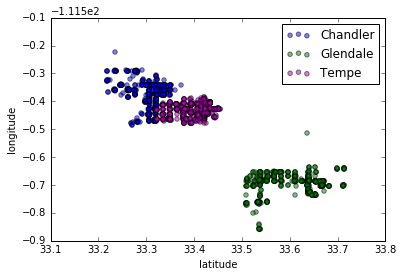
\includegraphics[keepaspectratio=true,scale=0.4]{./images/sub_location_plot}
\caption{Plot of location of reviews tagged to three cities in Phoenix}\label{fg:locations}
\end{figure}

For these different locations we see that to a greater or lesser extent, Sunday reviews receive the highest scores. We also see (focusing on the right hand line plot) that Chandler and Tempe receive roughly 5 and 10 reviews per day more than Glendale. The plot also uses the opacity of the dot to indicate numbers of reviews and there appears to be a trend that in the winter months (days of the year 200 through to 50), the Glendale area is particularly quiet (especially when comparing this to the other cities). Finally, we notice that Glendale appears to be a satellite city within Phoenix could be a possible reason for this.
\begin{figure}[H]
\centering
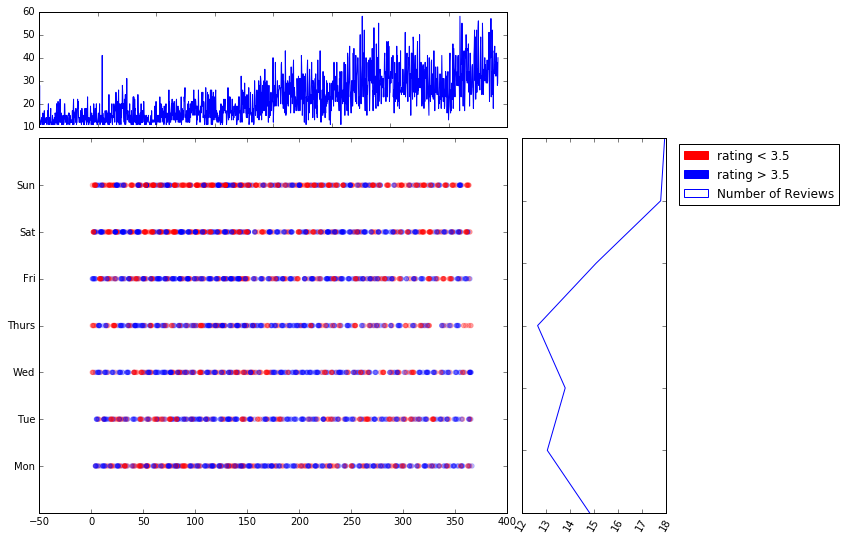
\includegraphics[keepaspectratio=true,scale=0.4]{./images/chandler_restaurants}
\caption{Plot of reviews above and below the mean for Restaurants in Chandler}\label{fg:chandler}
\end{figure}

\begin{figure}[H]
\centering
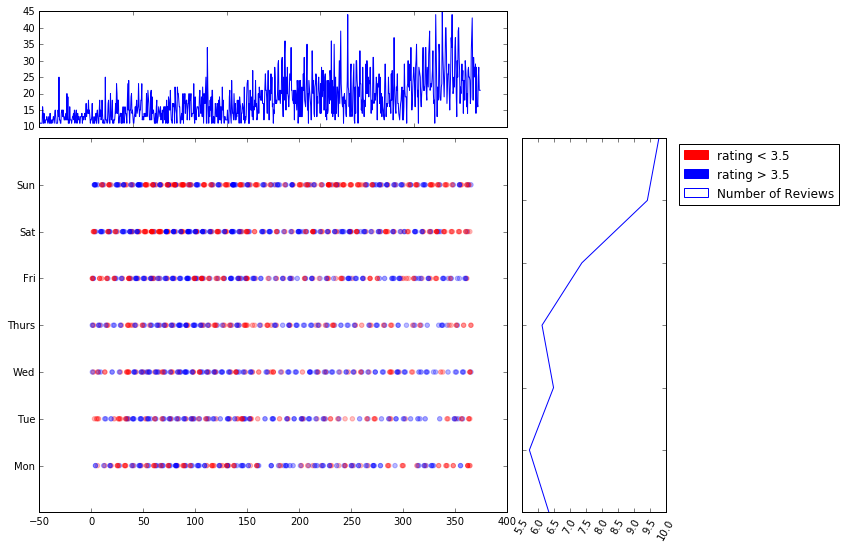
\includegraphics[keepaspectratio=true,scale=0.4]{./images/glendale_restaurants}
\caption{Plot of reviews above and below the mean for Restaurants in Glendale}\label{fg:glendale}
\end{figure}

\begin{figure}[H]
\centering
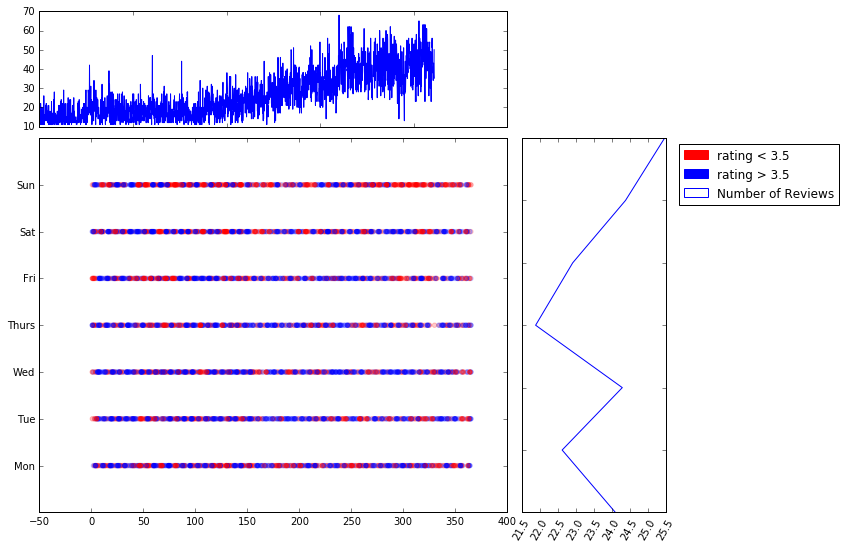
\includegraphics[keepaspectratio=true,scale=0.4]{./images/tempe_restaurants}
\caption{Plot of reviews above and below the mean for Restaurants in Tempe}\label{fg:tempe}
\end{figure}

We note that this location based study is likely to give us some insight into any seasonal and location based trends that are occurring within the restaurant businesses within the Phoenix area. Whether this information will only provide more qualitative information or if it will help us to refine our models by providing additional prior knowledge is to be explored further. Some additional source for future work is to focus on these trends and attempt to track specific categories of business as they become more or less popular.

\end{document}












